% !TEX program = xelatex
% 集创赛/IC设计 竞赛作品报告 LaTeX 模板
% 基于集创赛校赛答辩PPT + 初赛作品报告结构分析
% 编译方式：XeLaTeX

\documentclass[a4paper, 12pt]{article}

% ============================================================
% 中文支持（用 fontspec + xeCJK 替代 ctexart）
% ============================================================
\usepackage{fontspec}
\usepackage{xeCJK}
% 自动检测系统中文字体（STSong 没有粗体，用假粗体）
\setCJKmainfont[BoldFont={STSong},BoldFeatures={FakeBold=2}]{STSong}
\setCJKsansfont{STHeiti}
\setCJKmonofont{STFangsong}

% ============================================================
% 宏包导入
% ============================================================
\usepackage[margin=2.5cm]{geometry}          % 页面边距
\usepackage{graphicx}                        % 图片插入
\usepackage{booktabs}                        % 三线表
\usepackage{tabularx}                        % 自适应列宽表格
\usepackage{multirow}                        % 表格合并行
\usepackage{amsmath, amssymb}                % 数学公式
\usepackage{siunitx}                         % 单位 & 数值对齐
\usepackage{hyperref}                        % 超链接 & 书签
\usepackage{fancyhdr}                        % 页眉页脚
\usepackage{titlesec}                        % 标题样式
\usepackage{enumitem}                        % 列表样式
\usepackage{caption}                         % 图表标题
\usepackage{subcaption}                      % 子图
\usepackage{xcolor}                          % 颜色
\usepackage{listings}                        % 代码高亮
\usepackage{float}                           % 浮动体控制
\usepackage{appendix}                        % 附录
\usepackage{indentfirst}                     % 章节后首段也缩进

% ============================================================
% 颜色定义
% ============================================================
\definecolor{icblue}{RGB}{0, 70, 140}
\definecolor{icgray}{RGB}{100, 100, 100}

% ============================================================
% 超链接设置
% ============================================================
\hypersetup{
    colorlinks=true,
    linkcolor=icblue,
    citecolor=icblue,
    urlcolor=icblue
}

% ============================================================
% 页眉页脚
% ============================================================
\setlength{\headheight}{14pt}
\pagestyle{fancy}
\fancyhf{}
\fancyhead[L]{\small\leftmark}
\fancyhead[R]{\small\rightmark}
\fancyfoot[C]{\thepage}
\renewcommand{\headrulewidth}{0.4pt}

% ============================================================
% 标题格式
% ============================================================
\titleformat{\section}
  {\Large\bfseries\color{icblue}}{\thesection}{1em}{}
\titleformat{\subsection}
  {\large\bfseries}{\thesubsection}{1em}{}
\titleformat{\subsubsection}
  {\normalsize\bfseries}{\thesubsubsection}{1em}{}

% ============================================================
% 图表标题设置
% ============================================================
\captionsetup[figure]{labelsep=quad, font=small}
\captionsetup[table]{labelsep=quad, font=small}

% ============================================================
% 自定义命令
% ============================================================
% 芯片型号
\newcommand{\chip}[1]{\texttt{#1}}
% 关键指标高亮
\newcommand{\spec}[1]{\textbf{#1}}
% 接口定义表格列类型
\newcolumntype{L}[1]{>{\raggedright\arraybackslash}p{#1}}

% ============================================================
% 正文开始
% ============================================================
\begin{document}

% ============================================================
% 封面
% ============================================================
\begin{titlepage}
  \centering

  % 顶部留白
  \vspace*{2cm}

  % 集创赛 Logo
  
\includegraphics[width=0.18\textwidth]{fig/cicc_logo.png}

  \vspace{1cm}

  % 大赛名称
  {\LARGE\bfseries 第十届全国大学生集成电路创新创业大赛}

  \vspace{0.5cm}

  % 赛道
  {\Large 青软晶尊赛道}

  \vspace{2.2cm}

  % 作品名称（保持不变）
  {\LARGE\bfseries 基于tsmc40nm工艺的LDO芯片设计}

  \vspace{2.5cm}

  % 团队信息
  \begin{center}
  \renewcommand{\arraystretch}{1.8}
  {\large
  \begin{tabular}{rl}
    报告类型： & 仿真报告 / 设计报告  \\
    队伍编号： & CICCXXXXXXXX         \\
    团队名称： & 我boss得了mvp!                  \\
    指导教师： & XXX                  \\
  \end{tabular}
  }
  \end{center}

  \vfill

  % 底部日期
  {\Large\today}

  \vspace{1cm}
\end{titlepage}
\thispagestyle{empty}

\newpage

% ==================
% 目录
% ==================
\tableofcontents
\newpage

% ==================
% 1. 快速预览简介
% ==================
\section{快速预览简介}

% ---- 1.1 关键技术 ----
\subsection{关键技术}



% ---- 1.2 作品亮点 ----
\subsection{作品亮点}

\begin{itemize}[leftmargin=2em]
  \item \textbf{亮点一：} 极低的静态功耗，最小可达
  \item \textbf{亮点二：} 创新性放大器反馈结构，大幅提升系统的温漂系数，仅有（）
  \item \textbf{亮点三：} 1A大输出电流，2V宽输出范围
  \item \textbf{亮点四：} 采用了独特的误差放大器结构，大幅优化了psrr性能 
\end{itemize}

% ---- 1.3 指标说明 ----
\subsection{指标说明}

\begin{table}[H]
  \centering
  \caption{项目关键指标汇总}
  \label{tab:spec-summary}
  \begin{tabular}{clccc}
    \toprule
    序号 & 指标名称 & 前仿结果 & 后仿结果 & 项目需求 \\
    \midrule
    1 & 频率范围    & 1\textasciitilde1\,MHz & 1\textasciitilde1\,MHz & 1\textasciitilde1\,MHz \\
    2 & 占空比范围  & 1\%\textasciitilde99\%  & 1\%\textasciitilde99\%  & 1\%\textasciitilde99\%  \\
    3 & 温度稳定性  & $<$10\%                  & $<$10\%                  & $<$10\%                \\
    4 & 功耗        & $<$10\,mW                & $<$10\,mW                & 越小越好               \\
    \bottomrule
  \end{tabular}
\end{table}

% ==================
% 2. 模块接口说明
% ==================
\section{模块接口说明}

\begin{table}[H]
  \centering
  \caption{芯片引脚接口定义}
  \label{tab:pinout}
  \begin{tabular}{clcccp{4cm}}
    \toprule
    序号 & 接口名 & A/D & 电平 & I/O & 备注 \\
    \midrule
    1 & IN & A & 3.3 & I & 输入电压 \\
    2 & GND & A & 0 & I  & 地 \\
    3 & OUT & A & 0.8-2.8 & O  & 输出电压 \\
    4 & EN & D & 3.3/0  & I  & 使能输入 \\
    5 & TSD & D & 3.3/0  & O  & 过热输出 \\
    6 & OVC & D & 3.3/0  & O  & 过流输出 \\
    7 & CON & A & -  & I  & 控制电压 \\
    \bottomrule
  \end{tabular}
\end{table}

% ==================
% 3. 系统架构分析
% ==================
\section{系统架构分析}

\subsection{电路架构}

本作品使用传统LDO架构，包含电压基准、误差放大器、功率晶体管和反馈网络等核心模块。整体架构如图~\ref{fig:architecture}所示。

% 示例：插入架构框图
% \begin{figure}[H]
%   \centering
%   
\includegraphics[width=0.8\textwidth]{fig/architecture.pdf}
%   \caption{系统架构框图}
%   \label{fig:architecture}
% \end{figure}

根据图示，系统的误差放大器接受来自反馈网络的输出电压信号，并与电压基准进行比较，调整功率晶体管的导通程度以稳定输出电压。

\begin{gather}
  V_{fb} = V_{out} \\
  V_{out} = \frac{R_1+R_2+R_3}{R_2+R_3} V_{fb}
\end{gather}

或者

\begin{gather}
  V_{out} = \frac{R_3}{R_3+R_2} V_{fb}
\end{gather}

其中，$R_1$、$R_2$、$R_3$是反馈网络中的可调电阻。通过控制电阻阻值，即可输出较大的电压范围。

同时，系统包含过流保护和热关断功能以提高可靠性。系统可以通过外部控制接口调整输出电压和启停状态，满足不同应用场景的需求。

% ---- 模块1 ----
\subsection{模块一：电压基准}

本作品的电压基准模块采用经典的Bandgap基准设计，主要由启动电路、运放、温度补偿网络、电流镜和输出级组成。启动电路确保系统上电后能够正确进入工作状态；运放提供高增益以实现精确的电压比较；温度补偿网络利用PTAT电流和$V_{be}$特性实现低温漂；电流镜提供稳定的偏置电流；输出级则负责驱动后续模块。

\begin{figure}[H]
  \centering
  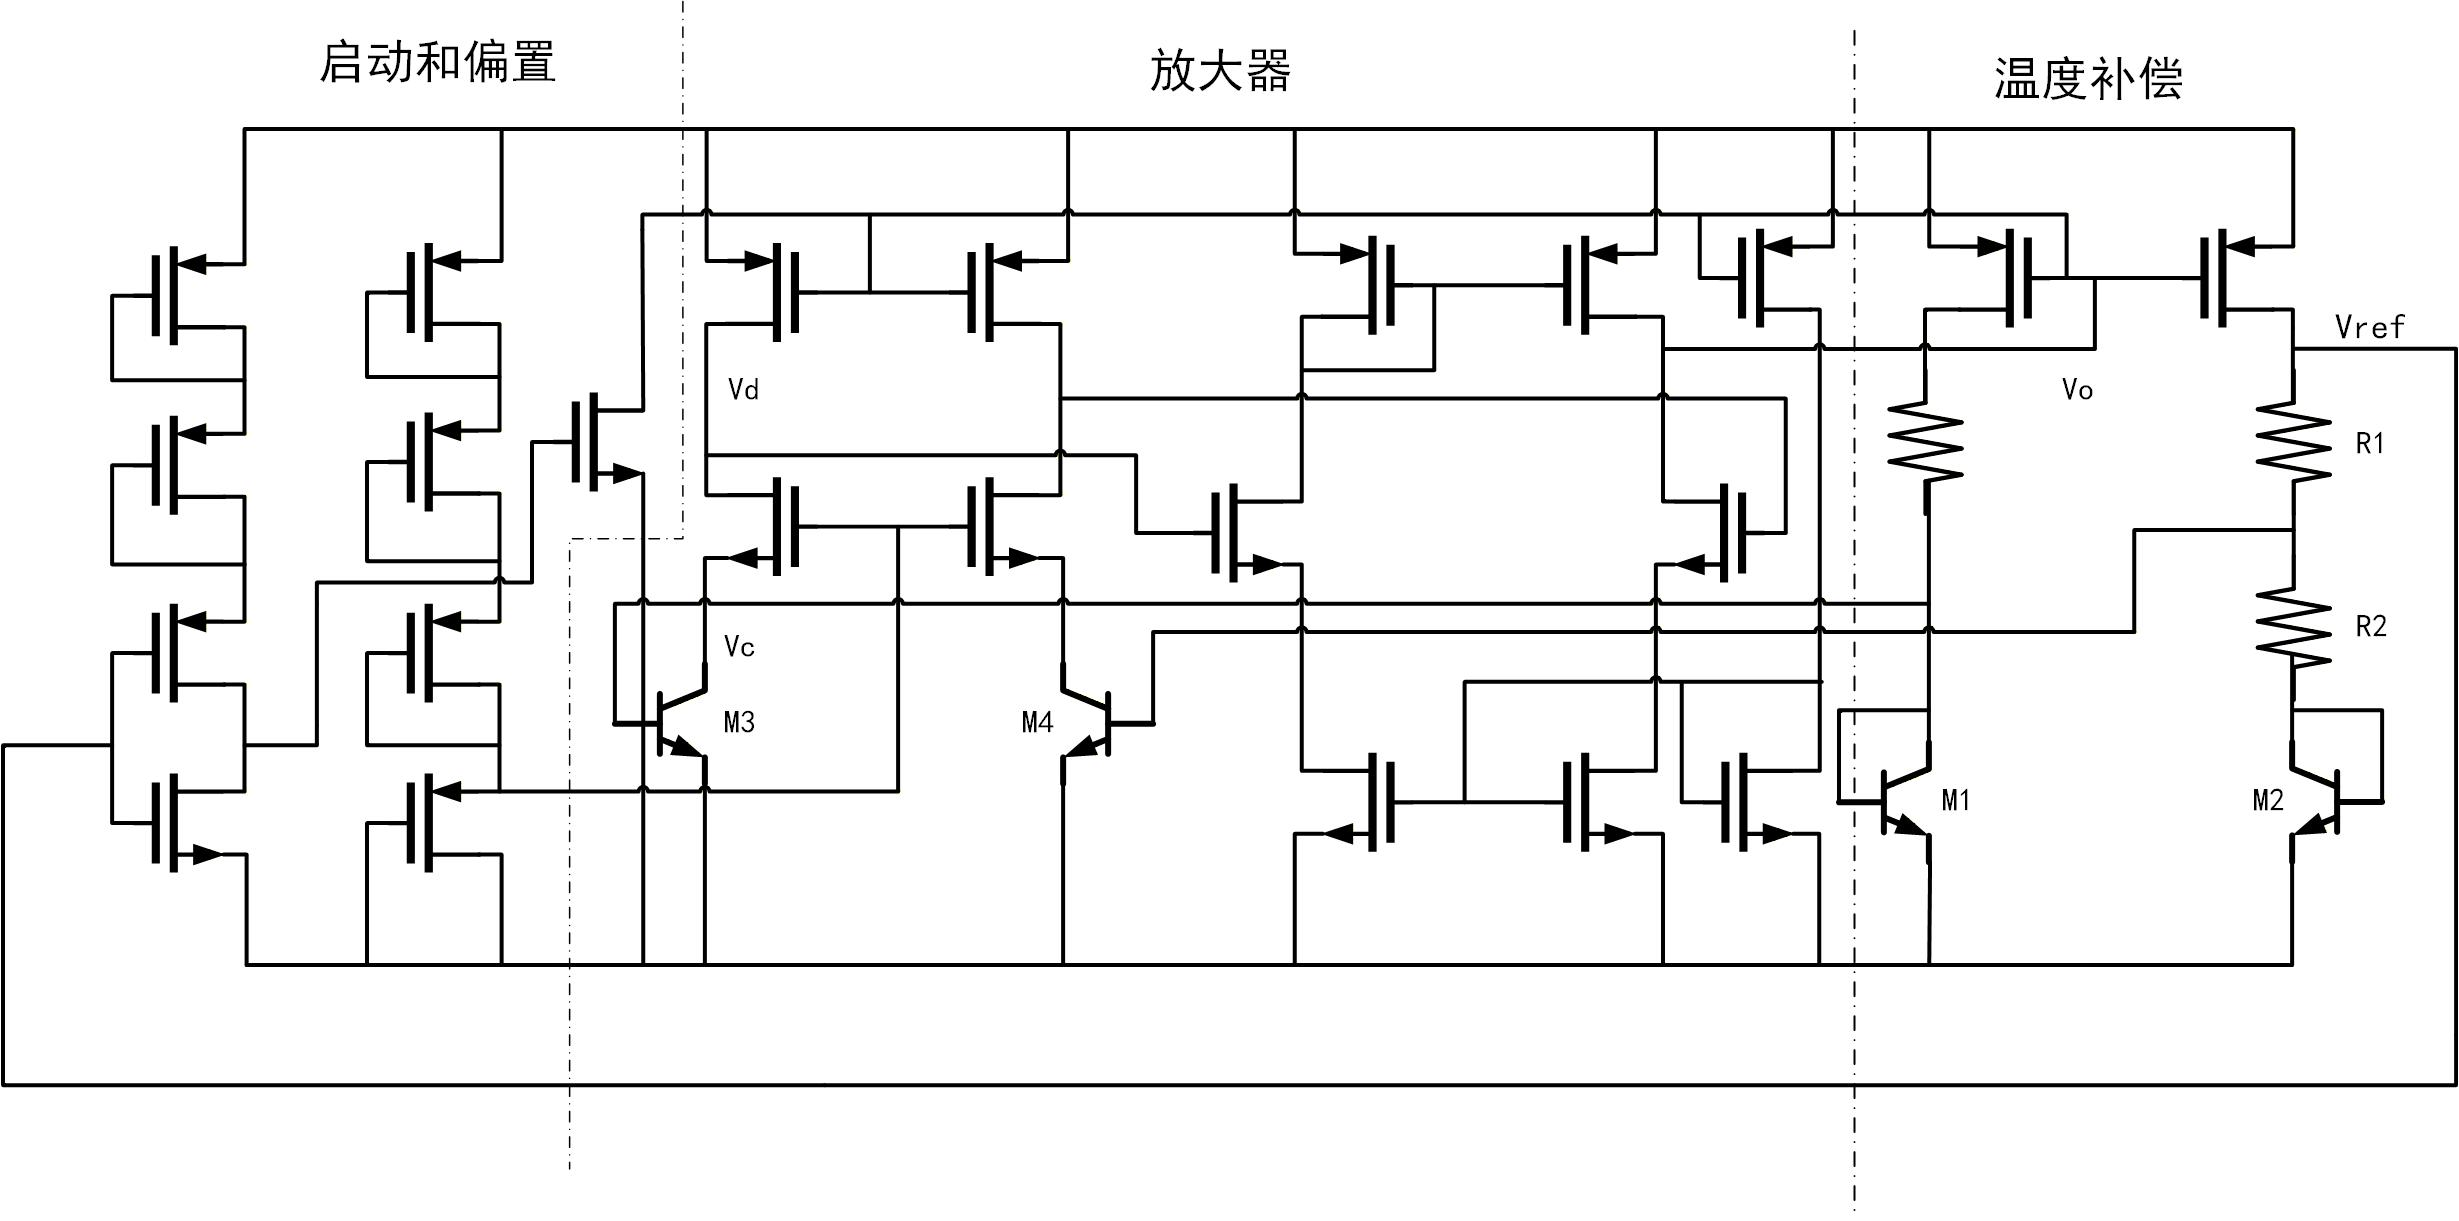
\includegraphics[width=1\textwidth]{fig/schematic/bandgap.jpg}
  \caption{电压基准模块示意图}
  \label{fig:bandgap-schematic}
\end{figure}

假定运放是理想的，根据电路，可知：

\begin{gather}
  V_{ref}=V_{be2}+R_{1}I_{ref} \\
  I_{ref}=I_{PTAT}=\frac{V_{be1}-V_{be2}}{R_2};
\end{gather}

根据

\begin{gather}
  V_{be} \approx V_{g0}-\frac{kT}{q}\ln{\frac{I}{I_s}}
\end{gather}

其中，$V_{g0}$是绝对零度时的硅能隙电压，$k$是玻尔兹曼常数，$T$是绝对温度，$q$是电子电荷量，$I$是电流，$I_s$是反向饱和电流。将上述方程代入式(1)和式(2)，可以得到：

\begin{gather}
  V_{ref}=V_{be2}+V_t\ln(n)*\frac{R_1}{R_2}
\end{gather}

其中，$n$是两个晶体管的面积比，$V_t=kt/q$是热电压。

对温度求偏导，可以得到：

\begin{gather}
  \frac{\partial V_{ref}}{\partial T}=\frac{\partial V_{be2}}{\partial T}+\frac{\partial V_t}{\partial T}\ln(n)*\frac{R_1}{R_2}
\end{gather}

再由
\begin{gather}
  \frac{\partial V_{be}}{\partial T} \approx -\frac{k}{q}\ln{\frac{I}{I_s}}+\frac{kT}{q}\frac{1}{I}\frac{\partial I}{\partial T}
\end{gather}

根据（1）-（10），令$\frac{\partial V_{be}}{\partial T}=0$可以得到

\begin{gather}
  \ln(n)*\frac{R_1}{R_2} \approx 17.2
\end{gather}

在设计中，我们取$n=8$，故：

\begin{gather}
  \frac{R_1}{R_2} \approx 8.27
\end{gather}

以上结果未考虑放大器的增益和电流镜的误差等非理想因素，实际设计中需要进行优化以达到更好的温度稳定性。

在本模块的设计中，本作品采用了一种新型的反馈方案。将输出电流反馈到运放的偏置端，形成一个负反馈回路。这种设计可以有效降低电压基准的输出噪声和温度漂移，提高系统的稳定性和可靠性。在多个反馈环路的配合下，系统能够在不同温度和工艺条件下保持稳定的输出电压，满足项目对温度稳定性的要求。

先考虑常规放大器的非理想特性对电路的影响，假设放大器的增益为$A$，输入失调电压为$V_{os}$，则电压基准的输出电压可以表示为：

\begin{gather}
  V_{ref} = V_{be1} + R_1 I_{ref} + V_{os} \\
  I_{ref} = \frac{V_{be1} + V_{os} - V_{be2}}{R_2}
\end{gather}

整理可得

\begin{gather}
    V_{ref} = V_{be1} + \frac{R_1}{R_2} (V_{be1} - V_{be2}) + \left(1 + \frac{R_1}{R_2}\right) V_{os}
\end{gather}

此时两边对温度进行求偏导，就会引入新的变量$\frac{\partial V_{os}}{\partial T}$，导致系统温漂系数不为零。

在典型结构中，放大器的输出端接电流镜给两个晶体管提供偏置电流。假定电流镜是理想的，输出电压$V_{ref}$相对稳定，即一侧电流镜的$V_{ds}$认为不变。此时，电流镜的栅极电压就等于$V_{os}*A$，根据$I_d$的表达式，可以整理到：

\begin{gather}
  V_{gs} = V_{os}*A - V_{in} \\
  I_d = \frac{1}{2} \mu C_{ox} \frac{W}{L} \left(V_{gs} - V_{th}\right)^2 \\
  I_d = \frac{1}{2} \mu C_{ox} \frac{W}{L} \left(V_{os}*A - V_{in} - V_{th}\right)^2
\end{gather}

再根据式（10），可以整理到：

\begin{gather}
  \frac{1}{2} \mu C_{ox} \frac{W}{L} \left(V_{os}*A - V_{in} - V_{th}\right)^2 = \frac{V_{be1} + V_{os} - V_{be2}}{R_2} \\
  C = \frac{1}{2} \mu C_{ox} \frac{W}{L}R_2 \\
  CA^2\left(V_{os}\right)^2 - 2CA\left(V_{in} + V_{th} + \frac{1}{2AC}\right) \left(V_{os}\right) + C\left(V_{in} + V_{th}\right)^2 - \left(V_{be1} - V_{be2}\right) = 0
\end{gather}

此时可以直观的看出$V_{os}$随增益的增大迅速减小，随增益的减小迅速增大。当然，也可以算出此时方程的解为：

\begin{gather}
  V_{os} = \frac{V_{in} + V_{th} + \frac{1}{2AC} \pm \sqrt{\left(V_{in} + V_{th} + \frac{1}{2AC}\right)^2 - \left(\left(V_{in} + V_{th}\right)^2 - \left(V_{be1} - V_{be2}\right)\right)}}{A}
\end{gather}

此时就可以直观的发现，在增益较小时，$V_{os}$会迅速增大；在增益提高时，$V_{os}$的会越来越小。在$R_2$较大时，C的数量级趋于1，此时$V_{os}$与$A$的关系趋近于反比例函数。$V_{os}$会极其依赖于增益。在80db时，$V_{os}$仍然有mV数量级，这大幅增加了系统的设计难度和功耗。

因此，我将电流镜的输出电流反馈回放大器，设计了全新的作用于bandgap的自偏置电路，有效提高了系统的温漂性能，降低了输入失调电压对系统温漂性能的影响，从而显著提升了系统的温度稳定性。

bandgap的放大器采用了两级差分放大器，其中第一级采用npn管作为输入，射级接地。bjt管的$V_{be}$和电流$I_c$的关系为：

\begin{gather}
  I_c = I_s e^{\frac{V_{be}}{V_t}} \\
  V_{be} = V_t \ln{\frac{I_c}{I_s}}
\end{gather}

其中，$I_s$是反向饱和电流。所以

\begin{gather}
  V_{be3} - V_{be4} = V_{os} = V_t \ln{\frac{I_{c3}}{I_s}} - V_t \ln{\frac{I_{c4}}{I_s}} = V_t \ln{\frac{I_{c3}}{I_{c4}}}
\end{gather}

同时，根据电路的偏置电流关系，考虑mos管的体效应，可以得到：

\begin{gather}
    V_{os} = V_{be3} - V_{be4} \\
    I_d = \frac{1}{2} \mu C_{ox} \frac{W}{L} \left(V_{os}*A - V_{in} - V_{th1}\right)^2\left(1 + \lambda_1 V_{dsp} \right) \\
    V_{dsp} = V_d - V_{in} \\
    I_d = \frac{1}{2} \mu C_{ox} \frac{W}{L} \left(V_{bias} - V_c - V_{th2}\right)^2\left(1 + \lambda_2 V_{dsn} \right) \\
    V_{dsn} = V_d - V_c \\
    I_d = I_c 
\end{gather}

其中，式（22）中的P管电流已经取绝对值，且$\lambda_1<0$，以保证$\lambda_1V_{dsp}>0$，所以可以求出：

\begin{gather}
  V_d = V_{in} + \frac{2I_d}{\lambda_1 \mu C_{ox} \frac{W}{L}\left(V_{os}*A-V_{in}-V_{th1}\right)^2} - \frac{1}{\lambda_1} \\
\end{gather}

故：

\begin{gather}
    V_{d1} - V_{d2} = \frac{2\left(I_{d1}-I_{d2}\right)}{\lambda_1 \mu C_{ox} \frac{W}{L}\left(V_{os}*A-V_{in}-V_{th1}\right)^2} \\
    V_{d1} - V_{d2} = \frac{2I_s\left(e^{\frac{V_{be3}}{V_t}} - e^{\frac{V_{be4}}{V_t}}\right)}{\lambda_1 \mu C_{ox} \frac{W}{L}\left(V_{os}*A-V_{in}-V_{th1}\right)^2}
\end{gather}

由于$\lambda_1 < 0$，所以$V_{d1} - V_{d2}$与$V_{be1} - V_{be2}$成反相关系。同时由于放大器极性的关系，$V_{out}$与$V_{d1} - V_{d2}$成正相关关系。所以系统此时引入了新的负反馈回路。



从另一个角度看，把两级放大器拆开来看，这个反馈回路结构就与bandgap中的相似，是将输出接到了电流镜的偏置端，对输入进行负反馈。

\begin{gather}
  V_{d1}-V_{d2} = V_{os2} \\
  V_{out} = V_{os2} A_2 
\end{gather}

第二级放大器是cascode差分输入、单端输出结构。其增益为：


通过将电流镜的输出电流反馈回放大器，设计了全新的作用于bandgap的自偏置电路，有效降低了放大器的失调电压对系统温漂性能的影响，从而显著提升了系统的温度稳定性。相比于传统结构和二阶bandgap，系统的温漂性能提升了一个数量级以上，并且还能保持不到5uA的静态电流，在tt工艺角下，系统的温漂系数仅有2.66093 ppm，满足项目对温度稳定性的要求。

此外，本模块还设计了有效的启动电路，在上电时注入启动电流，确保系统上电后能够正确进入工作状态。启动电路通过监测系统的电压和电流状态，在系统达到稳定工作条件时自动关闭，避免了不必要的功耗和潜在的稳定性问题。

% 示例：插入原理图
% \begin{figure}[H]
%   \centering
%   \begin{subfigure}[b]{0.48\textwidth}
%     \centering
%     \includegraphics[width=\textwidth]{fig/opa1_sch.pdf}
%     \caption{OPA1原理图}
%   \end{subfigure}
%   \hfill
%   \begin{subfigure}[b]{0.48\textwidth}
%     \centering
%     \includegraphics[width=\textwidth]{fig/opa2_sch.pdf}
%     \caption{OPA2原理图}
%   \end{subfigure}
%   \caption{电压比较器原理图}
%   \label{fig:opa_sch}
% \end{figure}

% ---- 模块2 ----
\subsection{模块二：误差放大器}

本作品的误差放大器采用两级结构，第一级采用折叠轨到轨外加共源级放大器，为系统提供足够的增益，第二级采用单位增益跟随器，为系统补偿零点的同时大幅改善了系统的psr性能。

\subsubsection{第一级放大器分析}

第一级放大器采用了折叠轨到轨结构，输入级采用了差分对称设计，能够实现输入电压的轨到轨范围内的线性放大。同时，输入级采用了共源级结构，能够提供较高的增益和较大的输出摆幅。

% ---- 模块3 ----
\subsection{模块三：限流模块}

限流模块采用电流镜结构实现过流保护功能。当输出电流超过设定阈值时，限流模块会迅速响应，将输出功率管快速关断，防止芯片损坏。该模块的设计重点在于提高响应速度和准确性，以确保在过流事件发生时能够及时保护系统。

限流模块的核心思路是将输出电流与一个预设的参考电流进行比较。当输出电流超过参考电流时，限流模块会触发保护机制，迅速降低输出电流至安全水平。为了实现这一功能，限流模块采用了高速比较器和快速响应的控制逻辑，以确保在过流事件发生时能够及时保护系统。此外，限流模块还具有可调节的参考电流设置，使得用户可以根据实际应用需求灵活调整过流保护的阈值，提高系统的适用性和可靠性。

% ---- 模块4 ----
\subsection{模块四：过温保护模块}

过温保护模块利用了三极管的$V_{be}$和bandgpa输出的PTAT电流特性实现温度检测。

% ---- 模块5 ----
\subsection{模块五：数字模块}



% ==================
% 4. 仿真结果
% ==================
\section{仿真结果}

\subsection{Bandgap模块}

对bandgap模块的仿真结果进行分析，验证其输出电压的稳定性、温度漂移特性以及上电状态的正确性。

tt、ss、ff三个工艺角下对输出电压的仿真结果如下：

\begin{figure}[H]
  \centering
  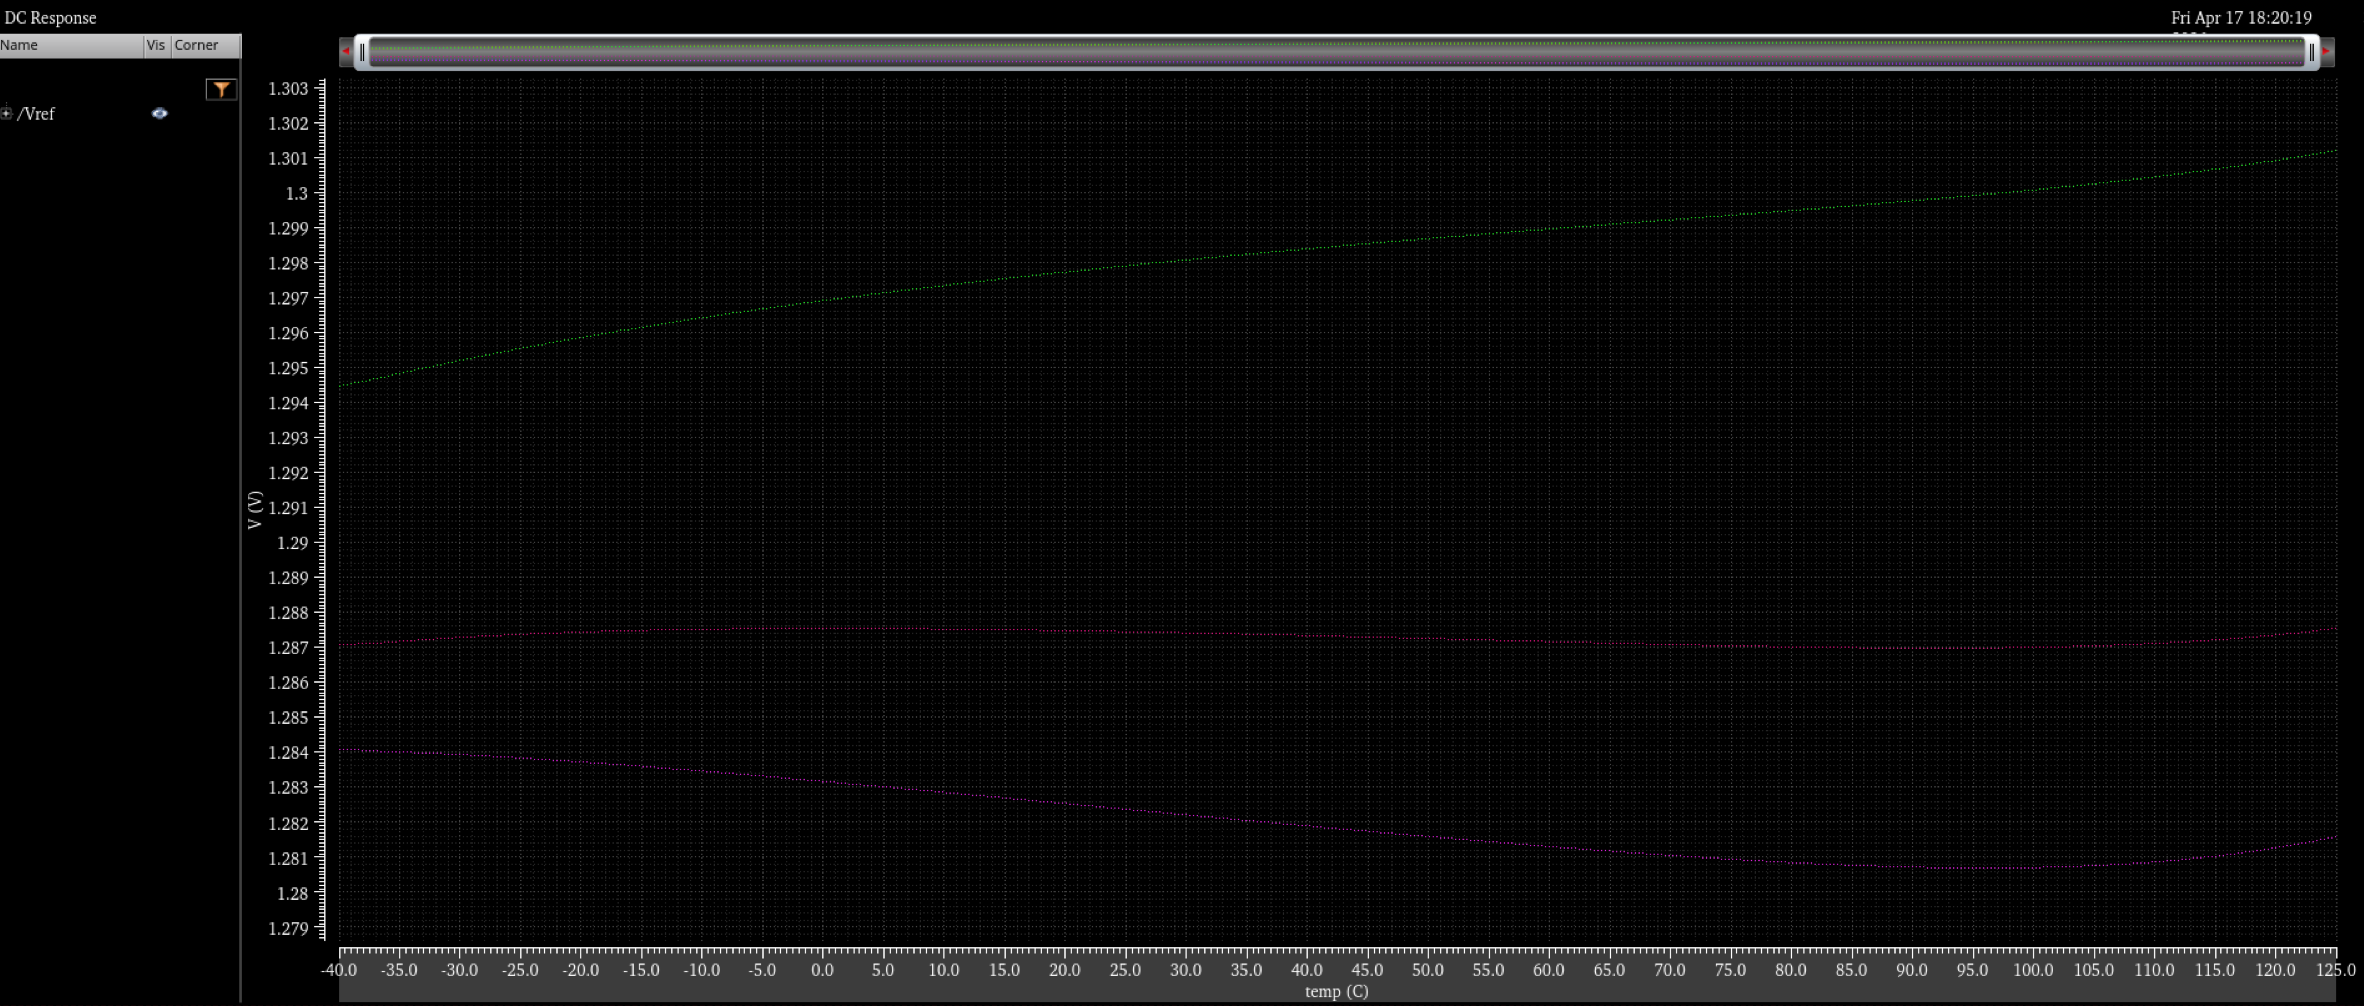
\includegraphics[width=0.8\textwidth]{fig/bandgap/bandgap_vref_noreverse.png}
  \caption{bandgap输出电压随温度变化的仿真结果}
  \label{fig:bandgap-temperature}
\end{figure}

\begin{figure}[H]
  \centering
  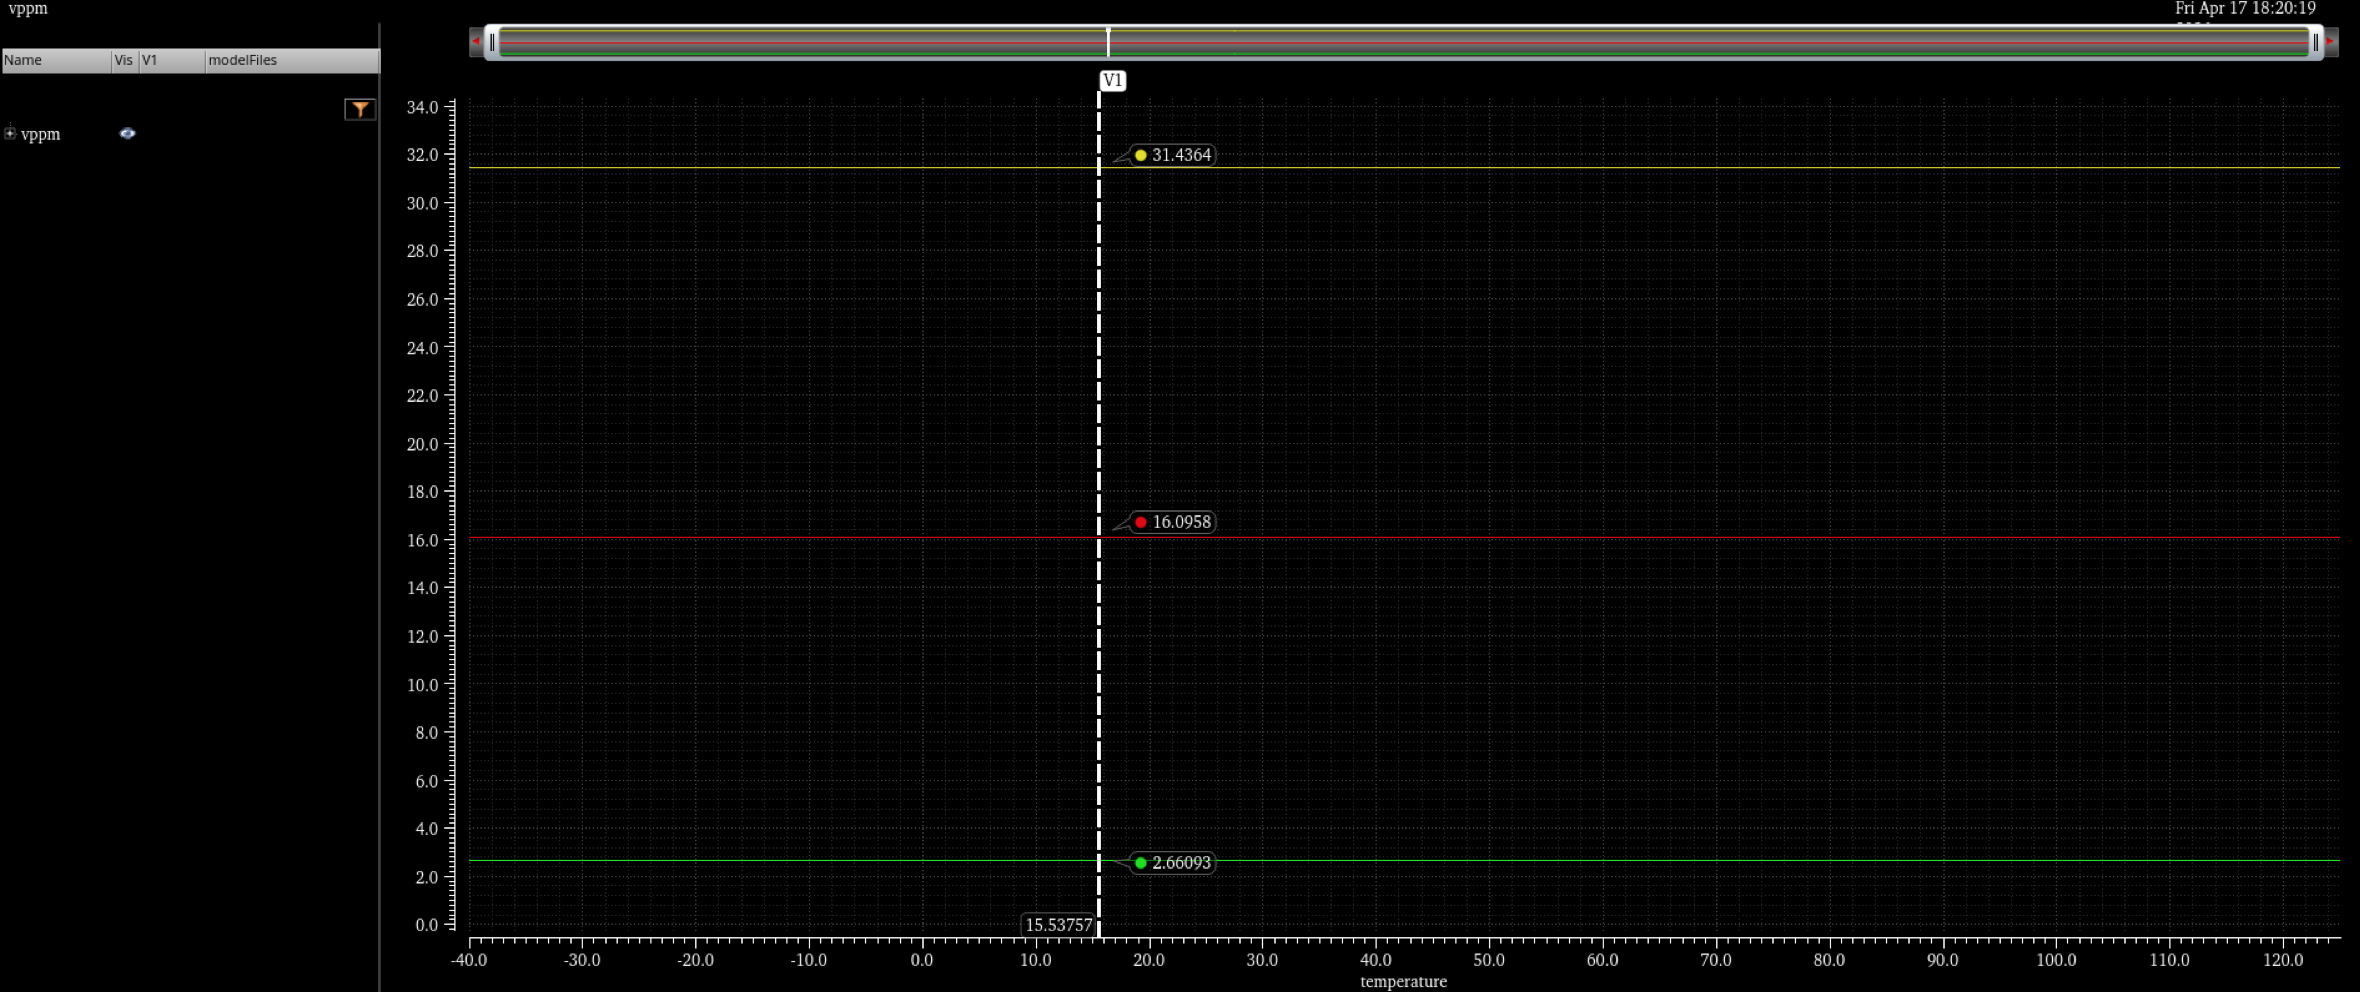
\includegraphics[width=0.8\textwidth]{fig/bandgap/bandgap_vppm_noreverse.png}
  \caption{bandgap输出温漂系数}
  \label{fig:bandgap-temperature-coeff}
\end{figure}

在tt、ss、ff三个工艺角下，-40、27、125三个温度下，对bandgap启动上电进行仿真，结果如下：

\begin{figure}[H]
  \centering
  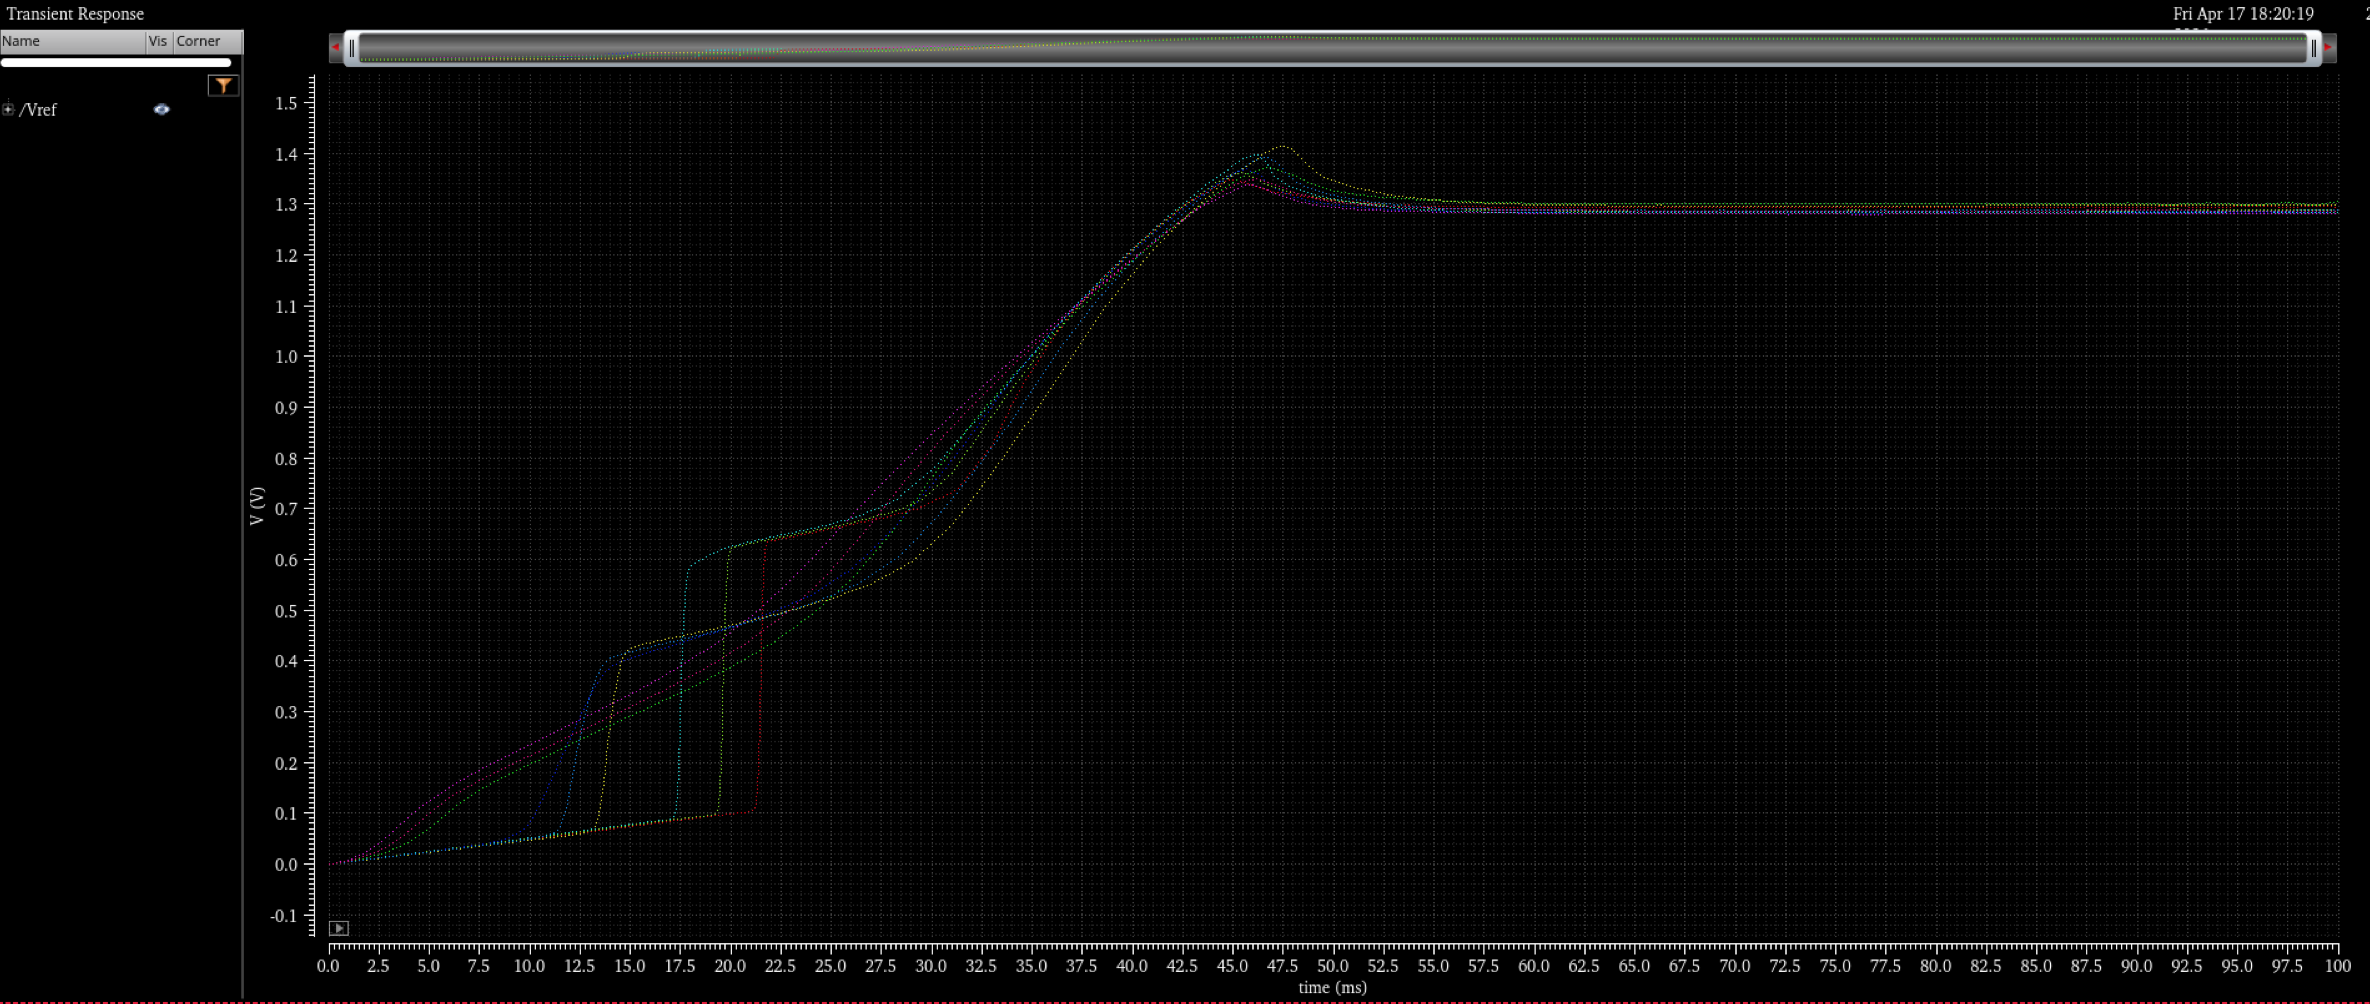
\includegraphics[width=0.8\textwidth]{fig/bandgap/bandgap_powerup_noreverse.png}
  \caption{bandgap上电仿真结果}
  \label{fig:bandgap-powerup}
\end{figure}

从上述仿真结果图可以得到bandgap的参数如下表：

% 示例：前仿结果
\begin{table}[H]
  \centering
  \caption{bandgap模块前仿关键指标}
  \label{tab:bandgap-pre}
  \begin{tabular}{lccc}
    \toprule
    指标 & tt & ss & ff \\
    \midrule
    温漂系数          & 2.66093 & 16.0958 & 31.4364 \\
    \bottomrule
  \end{tabular}
\end{table}

在tt工艺角下，系统的温漂系数仅为2.66093 ppm，表明系统具有极好的温度稳定性。

\begin{figure}[H]
  \centering
  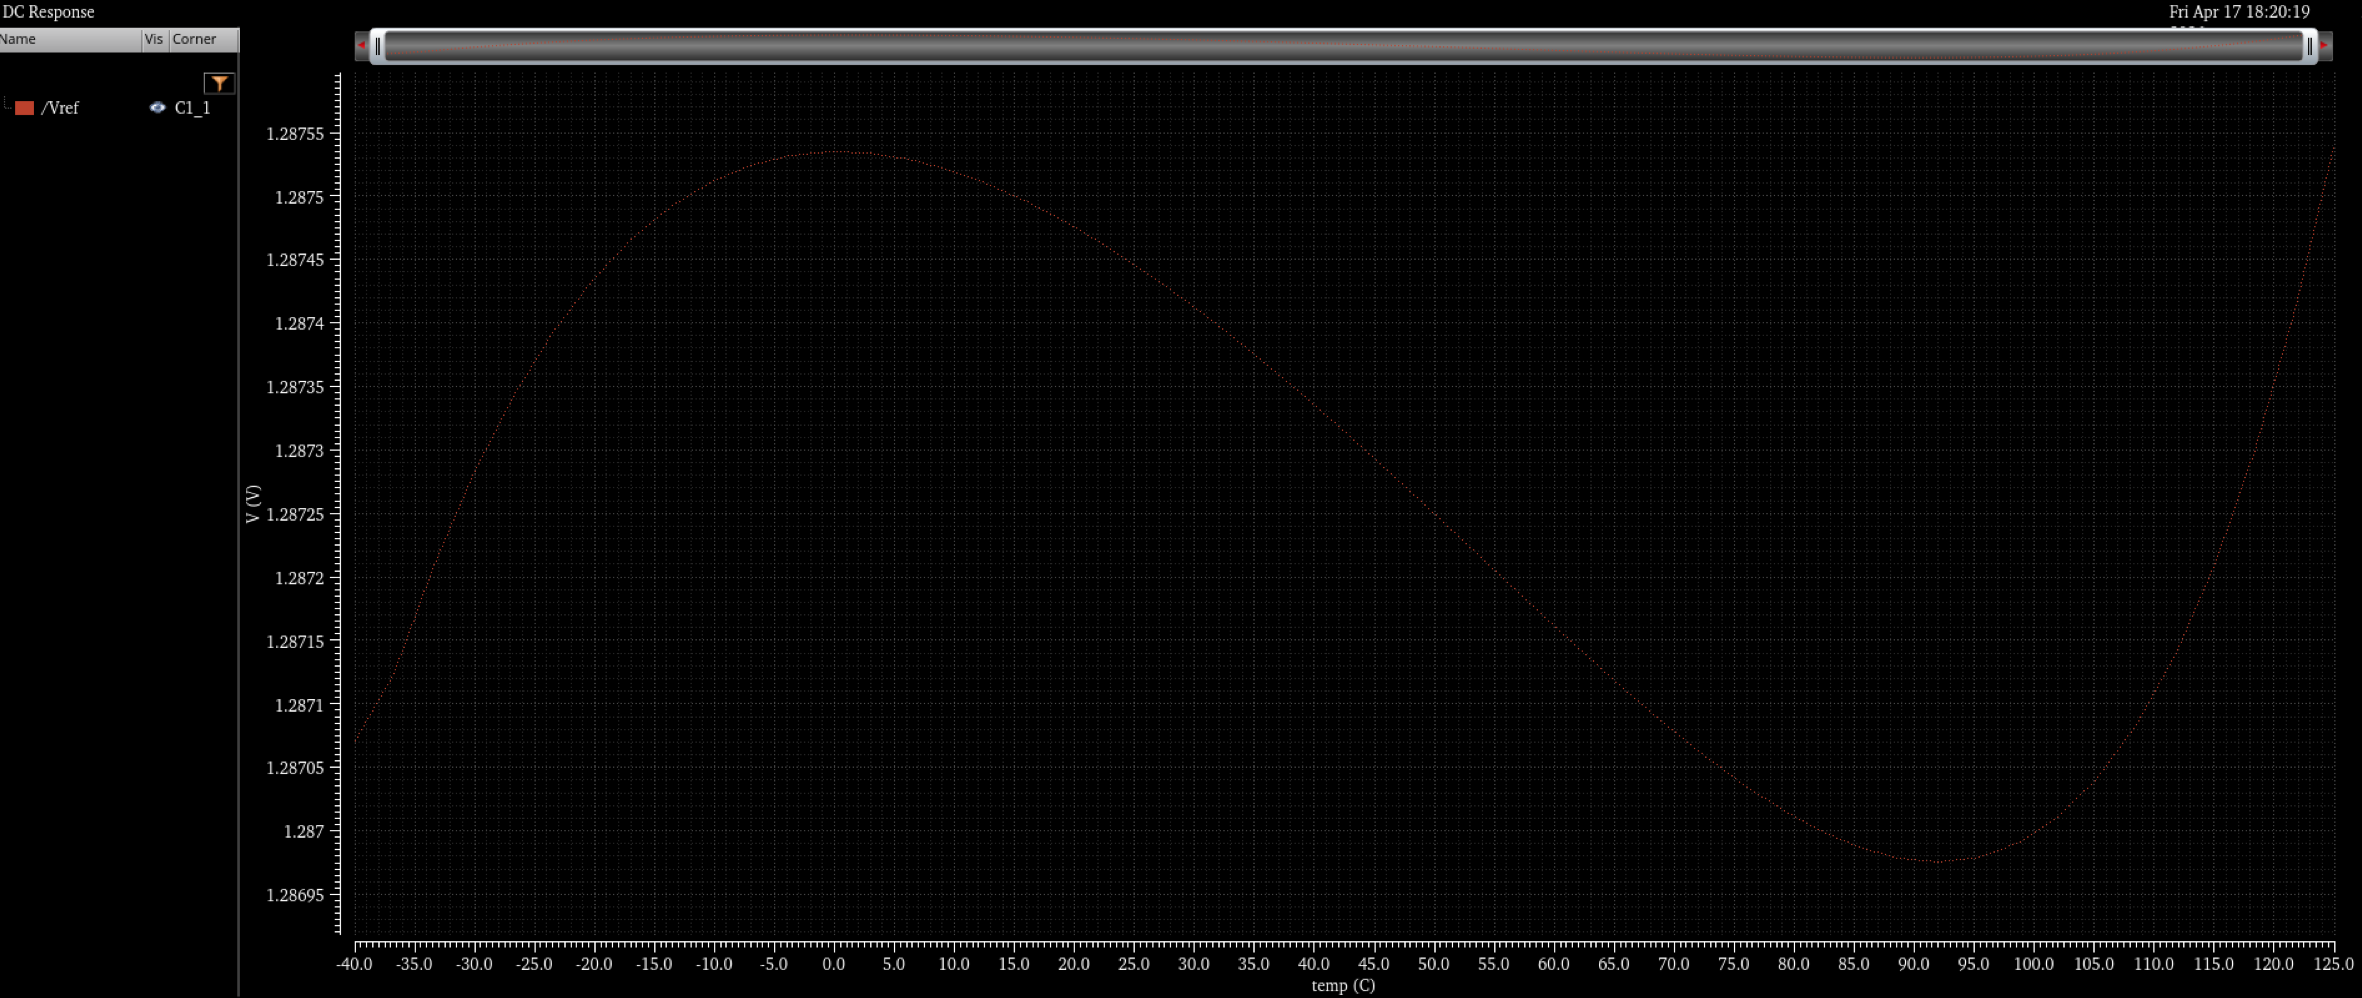
\includegraphics[width=0.8\textwidth]{fig/bandgap/bandgap_vref_tt_noreverse.png}
  \caption{bandgap在tt工艺角下的输出电压随温度变化的仿真结果}
  \label{fig:bandgap-temperature-tt}
\end{figure}

\subsection{主环路仿真结果}

系统主环路指的是系统的EA、功率管和反馈网络等核心模块的仿真结果。通过对主环路的仿真，可以验证系统的稳定性、频率响应、瞬态响应等关键性能指标。

本环节对系统主环路进行了dc、stb、ac仿真。在tt、ss、ff三个工艺角，-40、27、125三个温度下，系统输出电压1.8V，输出电流0、500mA、1A的情况下进行仿真。得到了系统的环路波特图、相位裕度、psr性能等关键指标的仿真结果。

\subsection{限流、过温保护、数字控制模块仿真结果}

系统还有限流、过温保护、数字控制模块，这些控制模块保护了电路在极端环境下的安全，增强了芯片的可拓展性。

过温保护模块的仿真结果展示出系统能够在温度逐渐升高到125以上时给出响应，关闭系统主要环路，降低输出电压，保护系统不受过热损害。并且在温度逐渐回落到125度一下时，重新打开系统的工作环路。

限流模块的仿真结果表明，当输出电流超过设定阈值时，系统能够及时触发过流保护机制，迅速关断输出管，降低输出电压，防止芯片损坏。

数字控制模块的仿真结果验证了系统能够通过外部控制接口调整输出电压和启停状态，满足不同应用场景的需求。

% 示例：插入仿真波形图
% \begin{figure}[H]
%   \centering
%   \begin{subfigure}[b]{0.48\textwidth}
%     \centering
%     \includegraphics[width=\textwidth]{fig/wave_3v.pdf}
%     \caption{$V_{CC}=3$\,V}
%   \end{subfigure}
%   \hfill
%   \begin{subfigure}[b]{0.48\textwidth}
%     \centering
%     \includegraphics[width=\textwidth]{fig/wave_5v.pdf}
%     \caption{$V_{CC}=5$\,V}
%   \end{subfigure}
%   \caption{不同电源电压下的输出波形}
%   \label{fig:output-wave}
% \end{figure}

\subsection{系统整体仿真结果}

完成了系统的每个模块仿真后，进行系统整体仿真，验证各模块协同工作时的性能表现。系统整体仿真包括dc、ac、stb等多种仿真类型，覆盖不同工艺角、温度和负载条件下的系统性能。

\subsubsection{电压输出能力}

通过对系统主环路电阻网络的调整，系统能够调整输出电压。仿真结果表明，在不同负载条件下，系统能够稳定输出预设的电压值，满足项目需求。

\subsubsection{电压输出精度}

根据电压输出能力的仿真结果，取$V_{outmax}$、$V_{outmin}$、1.8V三个电压值，tt、ss、ff三个工艺角下，输出电流0、500mA、1A，对温度从-40-125进行扫描，计算系统的输出电压精度。仿真结果表明，系统的输出电压精度满足项目需求，能够在不同工艺角和温度条件下保持稳定。

\subsubsection{系统psrr}

系统的psrr性能是衡量系统抗电源噪声能力的重要指标。通过对系统进行ac仿真，分析系统在不同频率下的psrr性能。取取$V_{outmax}$、$V_{outmin}$、1.8V三个电压值，tt、ss、ff三个工艺角下，输出电流0、500mA、1A，温度-40、27、125进行扫描。计算系统的psrr性能。仿真结果表明，系统的psrr性能满足项目需求，能够有效抑制电源噪声对输出电压的影响。此外，由于$V_{outmax}$无法满足psrr性能，我们还测试了可以在上述条件下保证psrr的$V_{outmax}^{'}$。

\subsubsection{系统功耗}

系统的功耗是衡量系统能效的重要指标。通过对系统进行dc仿真，分析系统在不同负载条件下的功耗表现。取$V_{outmax}$、$V_{outmin}$、1.8V三个电压值，tt、ss、ff三个工艺角下，输出电流0、500mA、1A，温度-40、27、125进行扫描。计算系统的功耗。仿真结果表明，系统的静态电流远远小于80uA，满足题目要求。

\subsubsection{系统保护功能}

系统的保护功能包括过流保护和过温保护。通过对系统进行dc仿真，输出电压在$V_{outmax}$、$V_{outmin}$、1.8V三个电压值下，tt、ss、ff三个工艺角下，温度-40、27、125的条件下，扫描负载电阻，得到系统的过流保护性能。在输出电压在$V_{outmax}$、$V_{outmin}$、1.8V三个电压值下，tt、ss、ff三个工艺角下，输出电流0、500mA、1A的条件下，扫描温度，得到系统的过温保护性能。仿真结果表明，系统的过流保护和过温保护功能能够在设定的阈值条件下及时响应，保护系统免受过流和过热损害。

% ==================
% 5. 版图设计
% ==================
\section{版图设计}

\subsection{版图规划}

描述版图的整体布局策略、对称性考虑、匹配方案等。

% 示例：插入版图
% \begin{figure}[H]
%   \centering
%   \includegraphics[width=0.7\textwidth]{fig/layout.pdf}
%   \caption{芯片整体版图}
%   \label{fig:layout}
% \end{figure}

\subsection{DRC/LVS验证}

% \begin{figure}[H]
%   \centering
%   \begin{subfigure}[b]{0.48\textwidth}
%     \centering
%     \includegraphics[width=\textwidth]{fig/drc.pdf}
%     \caption{DRC结果}
%   \end{subfigure}
%   \hfill
%   \begin{subfigure}[b]{0.48\textwidth}
%     \centering
%     \includegraphics[width=\textwidth]{fig/lvs.pdf}
%     \caption{LVS结果}
%   \end{subfigure}
%   \caption{设计规则验证}
%   \label{fig:drc-lvs}
% \end{figure}

\subsection{后仿验证}

描述版图寄生参数提取后的仿真结果，与前仿进行对比分析。

% ==================
% 6. 项目总结
% ==================
\section{项目总结}

\subsection{已完成工作}

\begin{enumerate}[leftmargin=2em]
  \item 完成了XXX模块的电路设计与仿真
  \item 完成了XXX模块的版图设计
  \item 完成了整体电路的前后仿验证
  \item \ldots
\end{enumerate}

\subsection{需要改进的部分}

\begin{itemize}[leftmargin=2em]
  \item 待改进项一
  \item 待改进项二
  \item \ldots
\end{itemize}

\subsection{后续工作}

\begin{enumerate}[leftmargin=2em]
  \item 整体版图连线及寄生参数提取
  \item 整体性能后仿
  \item 针对不足进行优化
  \item \ldots
\end{enumerate}

% ==================
% 参考文献
% ==================
\newpage
\bibliographystyle{IEEEtran}
% \bibliography{references}  % 取消注释并创建 references.bib 文件

% 临时使用手动文献列表
\section*{参考文献}
\addcontentsline{toc}{section}{参考文献}
\begin{enumerate}[leftmargin=2em, label={[\arabic*]}]
  \item NE555 datasheet, Texas Instruments.
  \item B. Razavi, \textit{Design of Analog CMOS Integrated Circuits}, 2nd ed., McGraw-Hill, 2017.
  \item P. R. Gray et al., \textit{Analysis and Design of Analog Integrated Circuits}, 5th ed., Wiley, 2009.
\end{enumerate}

% ==================
% 附录（可选）
% ==================
% \newpage
% \appendix
% \section{附录A：仿真参数设置}
% \section{附录B：模块网表}

\end{document}
